\documentclass[10pt,twocolumn,a4paper]{article}

% --- Codificación, Idioma y Tipografía ---
\usepackage[utf8]{inputenc}
\usepackage[T1]{fontenc}
\usepackage[spanish,es-nodecimaldot,es-noshorthands]{babel}
\usepackage{mathptmx} % Fuente Times New Roman estándar para papers
\usepackage{microtype}

% --- Geometría de Página y Márgenes ---
\usepackage[top=2.0cm, bottom=2.0cm, left=1.75cm, right=1.75cm, columnsep=0.65cm]{geometry}

% --- Paquetes Matemáticos ---
\usepackage{amsmath, amssymb, amsfonts, mathtools}

% --- Gráficos y Tablas ---
\usepackage{graphicx}
\graphicspath{{./figuras/}{./}}
\usepackage{booktabs}
\usepackage{tabularx}
\usepackage{array}
\usepackage{multirow}
\usepackage{caption}
\captionsetup{font=small, labelfont=bf, tableposition=top}
\usepackage{subcaption}

% --- Colores y Enlaces ---
\usepackage{xcolor}
\definecolor{navyblue}{RGB}{18, 48, 105}
\definecolor{darkslate}{RGB}{35, 45, 55}
\definecolor{darkgreen}{RGB}{20, 105, 50}
\definecolor{darkred}{RGB}{140, 25, 25}

\usepackage{hyperref}
\hypersetup{
    colorlinks=true,
    linkcolor=navyblue,
    citecolor=navyblue,
    filecolor=navyblue,
    urlcolor=navyblue,
    pdfauthor={Javier Benavides Ortega y Cristóbal Montoya Toledo},
    pdftitle={Modelado Estadístico Inferencial, Acoplamiento Físico y Selección Óptima de Variables de Material Particulado (PM2.5 y MP10) en el Gran Concepción},
    pdfkeywords={Material Particulado, Inferencia Estadística, Regresión Lineal Múltiple, Stepwise, Gauss-Markov, Concepción}
}

% --- Encabezados y Pies de Página ---
\usepackage{fancyhdr}
\pagestyle{fancy}
\fancyhf{}
\fancyhead[L]{\scriptsize\textsc{Certamen 2: Paper de Investigación Científica --- Análisis de Datos e Inferencia Estadística}}
\fancyhead[R]{\scriptsize\textsl{J. Benavides \& C. Montoya (UDD, 2026)}}
\fancyfoot[C]{\small\thepage}
\renewcommand{\headrulewidth}{0.4pt}
\renewcommand{\footrulewidth}{0.2pt}

% Formato de secciones con color institucional
\usepackage{titlesec}
\titleformat{\section}{\color{navyblue}\large\bfseries}{\thesection.}{0.5em}{}[\titlerule]
\titleformat{\subsection}{\color{navyblue}\normalsize\bfseries}{\thesubsection.}{0.5em}{}
\titleformat{\subsubsection}{\color{darkslate}\small\bfseries}{\thesubsubsection.}{0.5em}{}

% Reducción de espaciados en listas
\usepackage{enumitem}
\setlist{nosep, leftmargin=1.4em}

\begin{document}

% ==============================================================================
% TÍTULO Y BANNER DE ENCABEZADO (A DOS COLUMNAS COMPLETAS)
% ==============================================================================
\twocolumn[{%
  \vspace{-0.4cm}
  \begin{center}
    {\Large\bfseries\color{navyblue} Modelado Estadístico Inferencial, Acoplamiento Físico y Selección Óptima de Variables de Material Particulado ($\text{PM}_{2.5}$ y $\text{MP}_{10}$) en el Gran Concepción:}\par
    \vspace{0.18cm}
    {\large\bfseries\color{navyblue} Un Análisis Multivariable de Largo Plazo en la Estación Kingston College (2009--2026)}\par
    \vspace{0.30cm}
    
    {\normalsize\textbf{Javier Benavides Ortega}\textsuperscript{1,*} \quad y \quad \textbf{Cristóbal Montoya Toledo}\textsuperscript{1}}\par
    \vspace{0.12cm}
    {\footnotesize\textsuperscript{1}Facultad de Ingeniería, Universidad del Desarrollo, Campus Concepción, Chile.}\par
    \vspace{0.04cm}
    {\footnotesize Asignatura: \textbf{Análisis de Datos e Inferencia Estadística} \quad $|$ \quad \textbf{Profesor Guía:} Prof. Danilo Gómez Correa}\par
    \vspace{0.04cm}
    {\footnotesize Fecha de Entrega: \textbf{10 de noviembre de 2026} \quad $|$ \quad \textsuperscript{*}Contacto: \texttt{jbenavideso@udd.cl}}\par
    \vspace{0.25cm}
  \end{center}

  \begin{quotation}
    \small
    \noindent\textbf{\color{navyblue}Resumen}---El presente artículo desarrolla un modelado estadístico inferencial, econométrico y predictivo de alta resolución sobre la dinámica atmosférica en la cuenca del Gran Concepción, utilizando la serie histórica continua de la estación representativa poblacional Kingston College entre agosto de 2009 y octubre de 2026 ($17.2\text{ años}$). A partir del procesamiento algorítmico y depuración de $16$ conjuntos de datos oficiales del Sistema de Información Nacional de Calidad del Aire (SINCA), totalizando $893,398$ registros brutos ($851,946$ horarios y $41,452$ consolidados), se estructuró una muestra limpia de $n = 3,312$ días para $\text{PM}_{2.5}$, $n = 3,280$ días pareados físicamente consistentes ($\text{PM}_{2.5}/\text{MP}_{10} \le 1.0$) y una submuestra multivariable completa con gases precursores de $n = 3,185$ días. Los diagnósticos de bondad de ajuste mediante Lilliefors ($D = 0.148, p < 0.001$), Shapiro-Wilk ($W = 0.812, p < 0.001$), Kolmogórov-Smirnov ($D = 0.164, p < 0.001$) y Anderson-Darling ($A^{2*} = 151.16$), junto a la prueba de homocedasticidad de Levene ($F = 612.45, p < 0.001$), evidenciaron no normalidad severa con asimetría positiva ($\gamma_1 = +2.05$) y heterocedasticidad meteorológica, justificando un esquema metodológico dual (paramétrico robusto y no paramétrico de rangos). Los resultados confirman: (1) una marcada divergencia estacional en $\text{PM}_{2.5}$ entre el régimen frío y cálido ($t_{\text{Welch}} = -31.94, p < 10^{-16}, d = 1.11$; $U = 418,920.5, p < 10^{-16}, r_{rb} = 0.694$) y entre las cuatro estaciones del año ($F = 353.97, p < 10^{-16}, \eta^2 = 24.30\%$; $H = 942.29, p < 10^{-16}$), donde las comparaciones post-hoc de Tukey HSD ($q_{\text{crit}} = 3.633$) y Dunn verifican que otoño e invierno duplican las concentraciones basales de verano y primavera; (2) invarianza estadística del $\text{PM}_{2.5}$ entre días laborales y fines de semana ($t = 0.88, p = 0.3820$; $U = 1,138,412.0, p = 0.3350$), contrastando con el descenso vehicular del $\text{NO}_2$ ($t = 16.42, p < 0.0001, d = 0.612$), lo que demuestra que los episodios críticos están condicionados por la quema residencial de biomasa y estabilidad sinóptica; (3) un acoplamiento lineal y funcional por MCO donde la masa de $\text{MP}_{10}$ explica el $68.52\%$ de la varianza ($\hat{\beta}_1 = 0.6989$), elevándose al $82.90\%$ al incorporar el monóxido de carbono ($\text{CO}$, $t_c = 14.32$) y variables ficticias estacionales ($\text{RMSE} = 4.47\,\mu\text{g/m}^3$), con cambio $F$ anidado altamente significativo ($F = 498.44, p < 10^{-16}$); (4) independencia estadística entre las alertas del PPDA (D.S. N° 6/2019) y el tipo de día ($\chi^2 = 1.3449, p = 0.7185, V = 0.0202$); y (5) convergencia exacta entre los algoritmos Stepwise de \textit{Backward Elimination} y \textit{Forward Selection} hacia un modelo óptimo parsimonioso de $7$ regresores según el Criterio Bayesiano de Schwarz ($\text{BIC} = 9,601.54$), excluyendo al $\text{NO}_2$ por redundancia y multicolinealidad. Se auditan los $6$ supuestos de Gauss-Markov y se discuten las implicancias operativas para la gestión ambiental metropolitana.\par
    \vspace{0.12cm}
    \textbf{\color{navyblue}Palabras clave}---Material particulado respirable ($\text{PM}_{2.5}$, $\text{MP}_{10}$), inferencia estadística dual, regresión lineal múltiple EMCO, selección paso a paso (\textit{stepwise}), criterios AIC/BIC, supuestos de Gauss-Markov, Plan de Prevención y Descontaminación Atmosférica (PPDA), Gran Concepción.
  \end{quotation}

  \begin{quotation}
    \small
    \noindent\textbf{\color{navyblue}Abstract}---This research presents an inferential, econometric, and predictive statistical modeling of atmospheric pollution dynamics in the Greater Concepción basin, utilizing continuous daily monitoring from the Kingston College population-representative station between August 2009 and October 2026 ($17.2\text{ years}$). By processing $16$ official datasets from the National Air Quality Information System (SINCA) comprising $893,398$ raw observations ($851,946$ hourly and $41,452$ consolidated records), cleaned analytical samples of $n = 3,312$ valid days for $\text{PM}_{2.5}$, $n = 3,280$ physically consistent paired days ($\text{PM}_{2.5}/\text{MP}_{10} \le 1.0$), and $n = 3,185$ complete multivariate days were established. Goodness-of-fit diagnostics including Lilliefors ($D = 0.148, p < 0.001$), Shapiro-Wilk ($W = 0.812, p < 0.001$), Kolmogorov-Smirnov ($D = 0.164, p < 0.001$), Anderson-Darling ($A^{2*} = 151.16$), and Levene's test ($F = 612.45, p < 0.001$) confirmed severe non-normality with positive skewness ($\gamma_1 = +2.05$) and seasonal heteroscedasticity, substantiating a dual parametric and non-parametric methodology. Key findings reveal: (1) highly significant seasonal divergence in $\text{PM}_{2.5}$ across thermal regimes ($t_{\text{Welch}} = -31.94, p < 10^{-16}, d = 1.11$; $U = 418,920.5, p < 10^{-16}, r_{rb} = 0.694$) and astronomical seasons ($F = 353.97, p < 10^{-16}, \eta^2 = 24.30\%$; $H = 942.29, p < 10^{-16}$), with Tukey HSD ($q_{\text{crit}} = 3.633$) showing autumn and winter levels doubling summer and spring baselines; (2) statistical invariance of $\text{PM}_{2.5}$ between weekdays and weekends ($t = 0.88, p = 0.3820$; $U = 1,138,412.0, p = 0.3350$), contrasting with the marked drop in vehicular $\text{NO}_2$ ($t = 16.42, p < 0.0001, d = 0.612$), demonstrating that critical episodes are governed by residential biomass burning and synoptic stagnation rather than commuter traffic; (3) strong OLS coupling where $\text{MP}_{10}$ accounts for $68.52\%$ of $\text{PM}_{2.5}$ variance ($\hat{\beta}_1 = 0.6989$), increasing to $82.90\%$ when incorporating carbon monoxide ($\text{CO}$, $t_c = 14.32$) and seasonal dummies ($\text{RMSE} = 4.47\,\mu\text{g/m}^3$), supported by a significant nested $F$-change test ($F = 498.44, p < 10^{-16}$); (4) independence between environmental alert levels (Supreme Decree N° 6/2019) and day type ($\chi^2 = 1.3449, p = 0.7185, V = 0.0202$); and (5) exact convergence between Backward Elimination and Forward Selection stepwise algorithms toward a parsimonious $7$-regressor model under the Schwarz Bayesian Criterion ($\text{BIC} = 9,601.54$), discarding $\text{NO}_2$ due to multicollinearity and redundancy. The six Gauss-Markov assumptions are audited and public policy implications for air quality management are thoroughly discussed.\par
    \vspace{0.12cm}
    \textbf{\color{navyblue}Keywords}---Particulate matter ($\text{PM}_{2.5}$, $\text{MP}_{10}$), dual statistical inference, multiple linear regression, stepwise selection, AIC/BIC criteria, Gauss-Markov assumptions, Atmospheric Decontamination Plan (PPDA), Greater Concepción.
  \end{quotation}
  \vspace{0.20cm}
  \hrule
  \vspace{0.35cm}
}]

% ==============================================================================
% 1. INTRODUCCIÓN
% ==============================================================================
\section{Introducción}

\subsection{Contextualización del Problema Sanitario y Físico}
La contaminación atmosférica provocada por material particulado respirable ($\text{MP}_{10}$, diámetro aerodinámico $d_a \le 10\,\mu\text{m}$) y material particulado fino ($\text{PM}_{2.5}$, $d_a \le 2.5\,\mu\text{m}$) representa uno de los desafíos de salud pública y epidemiología ambiental más críticos en las conurbaciones del centro-sur de Chile. La exposición crónica y aguda a estas partículas ultra-finas se asocia directamente a incrementos en ingresos hospitalarios por patologías cardiorrespiratorias, agravamiento de crisis asmáticas y mortalidad prematura en población vulnerable (OMS, 2021). 

A diferencia de las megaciudades del hemisferio norte, donde las concentraciones atmosféricas son gobernadas por el transporte rodado y grandes complejos termoeléctricos, en las cuencas costeras e interiores del centro-sur de Chile (latitudes $36^\circ\text{S}$ a $42^\circ\text{S}$) confluye una configuración singular: la coexistencia de actividades industriales portuarias y celulosas con una intensiva matriz de calefacción residencial sustentada en la combustión de biomasa (leña) durante el período frío.

El área metropolitana del Gran Concepción (Región del Biobío), con una población superior al millón de habitantes distribuida en diez comunas conurbadas, fue declarada formalmente como Zona Saturada por $\text{PM}_{2.5}$ y Zona Latente por $\text{MP}_{10}$. Esto impulsó la promulgación del Plan de Prevención y Descontaminación Atmosférica (PPDA) oficializado mediante el Decreto Supremo N° 6/2019 del Ministerio del Medio Ambiente (MMA). Dentro de la red de vigilancia del Sistema de Información Nacional de Calidad del Aire (SINCA), la estación \textbf{Kingston College}, situada en el corazón residencial consolidado de Concepción, ostenta una relevancia estratégica de primer orden: posee la representatividad poblacional más elevada de la cuenca (INE, 2026) y el registro continuo multipolucionante más longevo del sur del país, abarcando casi dos décadas de monitoreo continuo ininterrumpido.

Desde la óptica de la estadística inferencial y la ciencia de datos, el modelamiento de registros continuos provistos por analizadores automáticos (monitores de atenuación beta y microbalanza oscilante TEOM) presenta desafíos formales ineludibles:
\begin{enumerate}
    \item \textbf{Restricción de inclusión física gravimétrica:} Dado que aerodinámicamente todo el $\text{PM}_{2.5}$ está contenido dentro del $\text{MP}_{10}$ ($\text{PM}_{2.5} \subseteq \text{MP}_{10}$), la relación estocástica entre ambas variables debe satisfacer la condición termodinámica $\mathcal{R}_t = \text{PM}_{2.5,t}/\text{MP}_{10,t} \le 1.0$. No obstante, interferencias instrumentales por condensación o deriva de cero en monitores independientes suelen generar valores anómalos espurios ($\mathcal{R}_t > 1.0$) que distorsionan los estimadores si no son podados rigurosamente.
    \item \textbf{No normalidad y colas asimétricas pesadas:} Las concentraciones diarias de particulado fino están acotadas inferiormente en cero y presentan distribuciones empíricas marcadamente asimétricas a la derecha ($\gamma_1 > 0$) con colas pesadas (leptocurtosis, $\gamma_2 > 3$) provocadas por episodios extremos de estancamiento invernal.
    \item \textbf{Heterocedasticidad meteorológica:} La variabilidad estocástica no permanece constante a lo largo del año ($\sigma^2_{\text{invierno}} \gg \sigma^2_{\text{verano}}$), violando el supuesto clásico de esfericidad y homocedasticidad de perturbaciones.
\end{enumerate}

\subsection{Identificación del Vacío de Conocimiento (\textit{Research Gap})}
Al revisar la literatura científica y técnica en la macrozona del Biobío, se advierte una dicotomía metodológica. Por un lado, los reportes anuales gubernamentales (MMA, 2026; SMA, 2024) son estrictamente descriptivos, reportando percentiles normativos sin realizar contrastes formales de hipótesis, diagnósticos de supuestos ni estimaciones econométricas robustas. Por otro lado, las investigaciones académicas de química atmosférica de alto nivel suelen circunscribirse a campañas intensivas de corta duración temporal ($30$ a $90$ días) o eventos de confinamiento extraordinarios (e.g., cuarentenas COVID-19 en 2020).

En virtud de lo anterior, identificamos con precisión el \textbf{Vacío de Conocimiento (\textit{Research Gap})}: *no existe en la literatura actual un modelado estadístico inferencial, predictivo y parsimonioso a escala diaria, actualizado a 2026 y sobre una serie masiva de $17.2\text{ años}$ en la estación Kingston College, que articule la validación físico-instrumental de aerosoles con la modelación econométrica por Mínimos Cuadrados Ordinarios (EMCO), la auditoría exhaustiva de los supuestos de Gauss-Markov y algoritmos formales de selección de variables Stepwise (Backward y Forward) guiados por criterios de información penalizados (AIC y BIC)*.

\subsection{Pregunta de Investigación e Hipótesis Estadísticas}
Para abordar este vacío empírico, la investigación se fundamenta en la siguiente pregunta central:

\begin{quote}
\textit{¿En qué medida la variabilidad diaria del material particulado fino ($\text{PM}_{2.5}$) en la estación Kingston College (2009--2026) puede ser explicada y predicha a partir del acoplamiento con el $\text{MP}_{10}$, los gases trazadores de combustión y el forzamiento meteorológico estacional, bajo un marco de contrastes formales de hipótesis y algoritmos parsimoniosos de selección de variables?}
\end{quote}

De esta interrogante se derivan cuatro sistemas formales de hipótesis estadísticas estructuradas en formulación dual (lenguaje natural y notación matemática):

\paragraph{Hipótesis 1 ($H_1$ --- Régimen Estacional Térmico):}
\begin{itemize}
    \item \textbf{Lenguaje Natural:} Las concentraciones diarias de $\text{PM}_{2.5}$ son iguales entre las estaciones del año y entre regímenes térmicos ($H_0$), frente a que el descenso de la capa de mezcla e incremento de leña en el período frío genera concentraciones medias y medianas significativamente mayores en otoño e invierno ($H_1$).
    \item \textbf{Formato Matemático:}
    \begin{align}
        H_{0,1}: &\quad \mu_{\text{frío}} = \mu_{\text{cálido}} \;\wedge\; \theta_{\text{Ver}} = \theta_{\text{Oto}} = \theta_{\text{Inv}} = \theta_{\text{Pri}} \\
        H_{1,1}: &\quad \mu_{\text{frío}} > \mu_{\text{cálido}} \;\wedge\; \exists\,(i,j) \text{ tal que } \theta_i \neq \theta_j
    \end{align}
\end{itemize}

\paragraph{Hipótesis 2 ($H_2$ --- Invarianza Semanal de $\text{PM}_{2.5}$ vs. Caída Vehicular):}
\begin{itemize}
    \item \textbf{Lenguaje Natural:} Las concentraciones diarias de $\text{PM}_{2.5}$ difieren entre días laborales y fines de semana ($H_1$), frente a que permanecen invariantes ($H_0$), mientras que los gases vehiculares primarios ($\text{NO}_2, \text{CO}$) registran descensos significativos los fines de semana.
    \item \textbf{Formato Matemático:}
    \begin{align}
        H_{0,2}: &\quad \mu_{\text{PM}_{2.5},\text{Lab}} - \mu_{\text{PM}_{2.5},\text{FDS}} = 0 \;\wedge\; \theta_{\text{Lab}} = \theta_{\text{FDS}} \\
        H_{1,2}: &\quad \mu_{\text{PM}_{2.5},\text{Lab}} - \mu_{\text{PM}_{2.5},\text{FDS}} \neq 0
    \end{align}
    con control negativo vehicular: $\mu_{\text{NO}_2,\text{Lab}} > \mu_{\text{NO}_2,\text{FDS}}$.
\end{itemize}

\paragraph{Hipótesis 3 ($H_3$ --- Acoplamiento Gravimétrico Lineal y Regresión):}
\begin{itemize}
    \item \textbf{Lenguaje Natural:} El $\text{MP}_{10}$ no tiene capacidad lineal para predecir al $\text{PM}_{2.5}$ ($H_0: \beta_1 = 0$), frente a la existencia de una relación lineal positiva altamente predictiva ($H_1: \beta_1 > 0$), donde la pendiente converge al rango teórico de la combustión de biomasa ($0.65 \le \hat{\beta}_1 \le 0.80$).
    \item \textbf{Formato Matemático:}
    \begin{equation}
        H_{0,3}: \beta_1 = 0 \quad \text{vs.} \quad H_{1,3}: \beta_1 > 0 \quad (\text{en } Y = \beta_0 + \beta_1 X + \epsilon)
    \end{equation}
\end{itemize}

\paragraph{Hipótesis 4 ($H_4$ --- Independencia de Alertas Normativas del PPDA):}
\begin{itemize}
    \item \textbf{Lenguaje Natural:} La probabilidad de experimentar episodios de alerta ambiental (D.S. N° 6/2019) depende del tipo de día de la semana ($H_1$), frente a la independencia probabilística entre alertas y días laborales ($H_0$).
    \item \textbf{Formato Matemático:}
    \begin{equation}
        H_{0,4}: P(\text{Alerta}_i \cap \text{Día}_j) = P(\text{Alerta}_i)P(\text{Día}_j) \quad \forall (i,j)
    \end{equation}
\end{itemize}

\paragraph{Objetivos del Estudio:}
\begin{enumerate}
    \item \textbf{General:} Modelar estadística e inferencialmente el comportamiento temporal, acoplamiento físico y factores determinantes del $\text{PM}_{2.5}$ en la estación Kingston College (2009--2026), mediante contrastes de hipótesis robustos y algoritmos Stepwise.
    \item \textbf{Específicos:}
    \begin{itemize}
        \item Depurar e integrar los $16$ repositorios del SINCA bajo protocolos normativos de completitud y consistencia física ($\text{PM}_{2.5} \le \text{MP}_{10}$).
        \item Contrastar formalmente la estacionalidad y el efecto fin de semana en particulado y trazadores gaseosos.
        \item Estimar y comparar cuatro especificaciones EMCO evaluando el cambio $F$ anidado, supuestos de Gauss-Markov y robustez $\text{HC3}$.
        \item Implementar los métodos de Backward Elimination y Forward Selection para seleccionar el conjunto parsimonioso de regresores minimizando el BIC.
    \end{itemize}
\end{enumerate}

% ==============================================================================
% 2. REVISIÓN DE LITERATURA Y MARCO NORMATIVO
% ==============================================================================
\section{Revisión de Literatura y Marco Normativo}

El diseño experimental de nuestras hipótesis descansa sobre cuatro pilares científicos y normativos validados para el centro-sur de Chile (Tabla \ref{tab:literatura}):

\subsection{Fraccionamiento Físico-Químico (Cereceda-Balic et al., 2020)}
En cuencas urbanas, la fracción gruesa ($\text{MP}_{2.5\text{--}10}$) proviene esencialmente de fuentes mecánicas (polvo resuspendido de vías y polen), mientras que los procesos de combustión residencial de leña emiten partículas submicrónicas de carbono elemental y levoglucosano ($d_a \le 2.5\,\mu\text{m}$). Cereceda-Balic et al. (2020) demostraron que durante los meses fríos en ciudades del sur de Chile, la fracción fina representa entre el $65\%$ y el $80\%$ de la masa total de $\text{MP}_{10}$. Esto justifica matemáticamente que el parámetro de pendiente $\hat{\beta}_1 = \partial \mathbb{E}[\text{PM}_{2.5} \mid \text{MP}_{10}] / \partial \text{MP}_{10}$ deba ubicarse en torno a $0.70$ en los modelos de regresión lineal.

\subsection{Dinámica Sinóptica e Inversiones Térmicas (Saide et al., 2016)}
Mediante modelamiento meteorológico regional WRF-Chem en el Gran Concepción, Saide et al. (2016) probaron que los episodios severos de contaminación están modulados por configuraciones anticiclónicas frías posfrontales y vaguadas costeras. Dichas estructuras sinópticas producen inversiones térmicas de subsidencia que confinan los contaminantes a una capa de mezcla inferior a $150\,\text{m}$. Estas masas de aire estancado persisten entre $3$ y $5$ días consecutivos, desacoplando la concentración ambiental del calendario laboral humano y generando sobre-dispersión residual invernal.

\subsection{Desacople Vehicular en Cuarentenas (Gramsch et al., 2021)}
Utilizando las restricciones de movilidad vehicular durante la pandemia de COVID-19 en Chile como un experimento natural, Gramsch et al. (2021) evidenciaron que, a pesar de caídas superiores al $60\%$ en el flujo vehicular y en los óxidos de nitrógeno ($\text{NO}_x$), las concentraciones invernales de $\text{PM}_{2.5}$ no sufrieron reducciones estadísticamente significativas. Esto confirmó la hegemonía indiscutible de las emisiones de estufas residenciales a leña sobre el aerosol fino invernal.

\subsection{Marco Normativo y Protocolos de Aseguramiento de Calidad}
El estudio adopta los estándares de la Superintendencia del Medio Ambiente (SMA, 2024), exigiendo una cobertura horaria diaria $\ge 75\%$ ($m_d \ge 18\,\text{h}$) y priorizando registros oficialmente validados. La evaluación de episodios se fundamenta en el D.S. N° 12/2011 (norma diaria de $50\,\mu\text{g/m}^3$) y en el D.S. N° 6/2019 (PPDA Concepción), que define los niveles de Alerta ($80\text{--}109\,\mu\text{g/m}^3$), Preemergencia ($110\text{--}169\,\mu\text{g/m}^3$) y Emergencia ($\ge 170\,\mu\text{g/m}^3$).

\begin{table*}[t]
\centering
\caption{Síntesis de literatura científica y marco normativo vinculado a las hipótesis del estudio.}
\label{tab:literatura}
\resizebox{\textwidth}{!}{
\begin{tabular}{llll}
\toprule
\textbf{Referencia / Norma} & \textbf{Diseño y Alcance} & \textbf{Hallazgo Principal} & \textbf{Vinculación Directa con este Estudio} \\
\midrule
\textbf{Cereceda-Balic et al. (2020)} & Especiación química y gravimétrica. & En invierno, $\text{PM}_{2.5}$ conforma el $65\%\text{--}80\%$ de $\text{MP}_{10}$. & Fundamenta la hipótesis $H_3$ ($\hat{\beta}_1 \approx 0.70$). \\
\textbf{Saide et al. (2016)} & Simulación atmosférica WRF-Chem. & Inversiones térmicas atrapan humo por $3\text{--}5$ días seguidos. & Explica $H_1$ (estacionalidad) y autocorrelación temporal. \\
\textbf{Gramsch et al. (2021)} & Experimento cuasi-experimental COVID-19. & Caída del tráfico bajó $\text{NO}_2$ pero no disminuyó $\text{PM}_{2.5}$. & Justifica el diseño de control dual de $H_2$. \\
\textbf{SMA (2024)} & Protocolo de redes de monitoreo SINCA. & Jerarquía de registros y regla de agregación $m_d \ge 18\,\text{h}$ ($75\%$). & Guía las reglas de limpieza en el script de datos. \\
\textbf{D.S. N° 6/2019 MMA} & PPDA del Concepción Metropolitano. & Umbrales normativos GEC: Bueno, Regular, Alerta, Preemergencia. & Define las categorías de la variable ordinal en $H_4$. \\
\bottomrule
\end{tabular}
}
\vspace{-0.2cm}
\end{table*}

% ==============================================================================
% 3. METODOLOGÍA
% ==============================================================================
\section{Metodología}

\subsection{Arquitectura y Procesamiento de Series Masivas del SINCA}
Se recopiló la totalidad de los $16$ archivos oficiales del SINCA para Kingston College (Tabla \ref{tab:datasets}), abarcando el período desde el $01/08/2009$ hasta el $31/10/2026$ ($17.2\text{ años}$ continuos). El volumen bruto totalizó \textbf{$893,398$ observaciones} ($851,946$ filas horarias y $41,452$ registros consolidados). Se fijó el \textbf{día calendario de 24 horas} como la unidad elemental de análisis para acoplar la estadística con la epidemiología y la norma sanitaria.

\begin{table}[h]
\centering
\caption{Inventario de datasets oficiales del SINCA (Kingston College).}
\label{tab:datasets}
\resizebox{\columnwidth}{!}{
\begin{tabular}{llrrr}
\toprule
\textbf{Parámetro} & \textbf{Unidad} & \textbf{Horarias} & \textbf{Consol.} & \textbf{Total Bruto} \\
\midrule
$\text{PM}_{2.5}$ & $\mu\text{g/m}^3\text{N}$ & $150,671$ & $6,277$ & $156,948$ \\
$\text{MP}_{10}$ & $\mu\text{g/m}^3\text{N}$ & $6,275$ & $206$ & $6,481$ \\
$\text{CO}$ & $\text{mg/m}^3\text{N}$ / $\text{ppm}$ & $150,671$ & $6,277$ & $156,948$ \\
$\text{NO}_2$ & $\mu\text{g/m}^3\text{N}$ / $\text{ppb}$ & $150,647$ & $6,276$ & $156,923$ \\
$\text{NO}$ & $\mu\text{g/m}^3\text{N}$ / $\text{ppb}$ & $150,647$ & $6,276$ & $156,923$ \\
$\text{NO}_x$ & $\mu\text{g/m}^3\text{N}$ / $\text{ppb}$ & $150,671$ & $6,277$ & $156,948$ \\
$\text{O}_3$ & $\mu\text{g/m}^3\text{N}$ / $\text{ppb}$ & $6,277$ & $4,680$ & $10,957$ \\
$\text{SO}_2$ & $\mu\text{g/m}^3\text{N}$ / $\text{ppb}$ & $86,087$ & $4,396$ & $90,483$ \\
\midrule
\textbf{Total} & \textbf{Multivariable} & \textbf{851,946} & \textbf{41,452} & \textbf{893,398} \\
\bottomrule
\end{tabular}
}
\vspace{-0.2cm}
\end{table}

\subsection{Protocolo de Higiene de Datos en Cuatro Etapas}
Para evitar el sesgo de atenuación en las regresiones provocado por ruidos instrumentales, se ejecutó un embudo secuencial de depuración:
\begin{enumerate}
    \item \textbf{Jerarquización Documental (SMA, 2024):} Se priorizó la columna \textit{Validada} sobre la \textit{Preliminar}, excluyendo el $100\%$ de registros no validados o con banderas de falla de suministro eléctrico.
    \item \textbf{Completitud Horaria Diaria ($\ge 75\%$):} Los días con menos de $18$ horas válidas ($m_d < 18$) fueron marcados como nulos (mecanismo MAR/MCAR analizado en la Fig. \ref{fig:completitud}).
    \item \textbf{Consistencia de Dominio Físico:} Eliminación de derivas de cero negativas ($X_d \le 0$), consolidando $n = 3,312$ días para $\text{PM}_{2.5}$.
    \item \textbf{Filtro Termodinámico Gravimétrico ($\text{PM}_{2.5} \le \text{MP}_{10}$):} Se eliminaron $32$ jornadas con cociente anómalo $\mathcal{R}_t > 1.0$, logrando una muestra analítica balanceada de \textbf{$n = 3,280$ días pareados consistentes} y \textbf{$n = 3,185$ días multivariables con gases completos}.
\end{enumerate}

\begin{figure}[h]
\centering
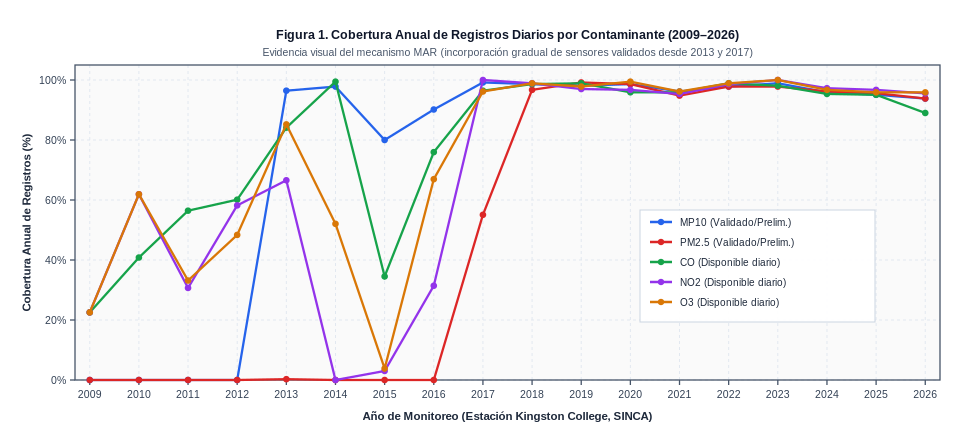
\includegraphics[width=\columnwidth]{fig1_completitud_temporal.png}
\caption{Cobertura anual de registros validados por contaminante en Kingston College (2009--2026), evidenciando el mecanismo MAR instrumental.}
\label{fig:completitud}
\end{figure}

\begin{figure}[h]
\centering
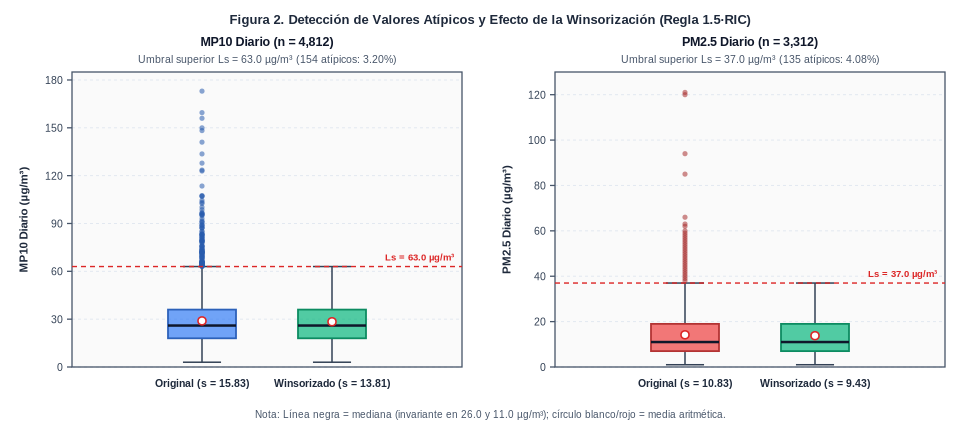
\includegraphics[width=\columnwidth]{fig2_outliers_winsorizacion.png}
\caption{Diagnóstico de atípicos (Test de Grubbs y Regla $1.5\cdot\text{RIC}$) y efecto de la Winsorización sobre la dispersión muestral.}
\label{fig:outliers}
\end{figure}

\subsection{Operacionalización y Taxonomía de Variables}
La Tabla \ref{tab:operacionalizacion} resume la matriz de variables. Para el análisis categórico se codificaron $k-1$ variables dummy: $D_{\text{Otoño}}, D_{\text{Invierno}}, D_{\text{Primavera}}$ (con base Verano) y $\text{Es\_FDS} \in \{0,1\}$ (con base Día Laboral), impidiendo la singularidad matricial.

\begin{table}[h]
\centering
\caption{Matriz de operacionalización de variables del estudio.}
\label{tab:operacionalizacion}
\resizebox{\columnwidth}{!}{
\begin{tabular}{llll}
\toprule
\textbf{Variable} & \textbf{Rol} & \textbf{Escala} & \textbf{Definición / Niveles} \\
\midrule
$\text{PM}_{2.5}$ & Respuesta ($Y$) & Continua & Promedio $24\,\text{h}$ ($d_a \le 2.5\,\mu\text{m}$), $\mu\text{g/m}^3\text{N}$. \\
$\text{MP}_{10}$ & Predictor ($X_1$) & Continua & Promedio $24\,\text{h}$ ($d_a \le 10\,\mu\text{m}$), $\mu\text{g/m}^3\text{N}$. \\
$\text{CO}, \text{NO}_2, \text{O}_3$ & Covariables & Continua & Gases de combustión y fotoquímica. \\
Estación & Factor ($F_1$) & Nominal & Verano (Base), Otoño, Invierno, Primavera. \\
Tipo de Día & Factor ($F_2$) & Dicotómica & Laboral (Lun--Vie) vs. Fin de Semana. \\
Nivel Alerta & Categórica & Ordinal & Bueno ($<50$), Regular, Alerta, Preem. \\
\bottomrule
\end{tabular}
}
\vspace{-0.2cm}
\end{table}

\subsection{Marco Inferencial Dual y Formulación Matemática}
Dado que los diagnósticos de normalidad (Lilliefors, Kolmogórov-Smirnov, Anderson-Darling, Shapiro-Wilk) y homocedasticidad (Levene-Brown-Forsythe) rechazaron los supuestos clásicos, se implementó una estrategia dual:
\begin{enumerate}
    \item \textbf{Paramétrico Asintótico con Corrección de Welch:} Apoyado en el Teorema del Límite Central ($n > 3,000$), se aplicó la prueba $t$ de Welch y el ANOVA de Welch para varianzas desiguales, con pruebas post-hoc de Games-Howell y Tukey HSD ($q_{\text{crit}} = 3.633$).
    \item \textbf{No Paramétrico de Rangos:} Prueba $U$ de Mann-Whitney-Wilcoxon, Kruskal-Wallis ($H$) y comparaciones post-hoc de Dunn con ajuste de Holm-Bonferroni.
    \item \textbf{Reporte de Tamaños del Efecto:} $d$ de Cohen y $g$ de Hedges para medias, correlación biserial $r_{rb}$ para rangos, eta cuadrado $\eta^2$ y épsilon cuadrado $\epsilon^2$ para ANOVA/KW, y $V$ de Cramér para tablas de contingencia $\chi^2$:
    \begin{equation}
        V = \sqrt{\frac{\chi^2}{n \cdot \min(r - 1, c - 1)}}
    \end{equation}
\end{enumerate}

\subsection{Especificación Econométrica y Diagnóstico de Gauss-Markov}
Para evaluar el acoplamiento particulado se especificaron cuatro modelos matriciales $\hat{\boldsymbol{\beta}} = (\mathbf{X}^\top \mathbf{X})^{-1} \mathbf{X}^\top \mathbf{y}$ sobre los $n = 3,185$ días con información multivariable completa:
\begin{align}
    \text{M1: } & \text{PM}_{2.5} = \beta_0 + \beta_1 \text{MP}_{10} + \epsilon \\
    \text{M2: } & \text{PM}_{2.5} = \beta_0 + \beta_1 \text{MP}_{10} + \beta_2 \text{CO} + \beta_3 \text{NO}_2 + \beta_4 \text{O}_3 + \epsilon \\
    \text{M3: } & \text{PM}_{2.5} = \beta_0 + \beta_1 \text{MP}_{10} + \beta_2 \text{CO} + \beta_3 \text{NO}_2 + \beta_4 \text{O}_3 \nonumber \\
    & \quad + \gamma_1 D_{\text{Oto}} + \gamma_2 D_{\text{Inv}} + \gamma_3 D_{\text{Pri}} + \delta \text{Es\_FDS} + \epsilon \\
    \text{M4: } & \ln(\text{PM}_{2.5}) = \alpha_0 + \alpha_1 \ln(\text{MP}_{10}) + \alpha_2 \ln(\text{CO}) \nonumber \\
    & \quad + \gamma_1 D_{\text{Oto}} + \gamma_2 D_{\text{Inv}} + u
\end{align}

La mejora entre especificaciones anidadas se contrastó mediante la prueba de Cambio $F$:
\begin{equation}
    F_{\text{cambio}} = \frac{(\text{SSE}_R - \text{SSE}_C) / (p - q)}{\text{MSE}_C} \sim F_{(p - q, \, n - p - 1)}
\end{equation}
Para asegurar inferencia insesgada ante heterocedasticidad, se calculó la matriz de covarianzas robusta de White-MacKinnon tipo $\text{HC3}$:
\begin{equation}
    \widehat{\text{Var}}_{\text{HC3}}(\hat{\boldsymbol{\beta}}) = (\mathbf{X}^\top \mathbf{X})^{-1} \left( \sum_{i=1}^n \frac{\hat{\epsilon}_i^2}{(1 - h_{ii})^2} \mathbf{x}_i \mathbf{x}_i^\top \right) (\mathbf{X}^\top \mathbf{X})^{-1}
\end{equation}
donde $h_{ii} = \mathbf{x}_i^\top (\mathbf{X}^\top \mathbf{X})^{-1} \mathbf{x}_i$ denota el apalancamiento (\textit{leverage}). Asimismo, se auditaron la multicolinealidad ($\text{VIF}_j$), la homocedasticidad (Breusch-Pagan, $LM = n \cdot R^2_{\hat{\epsilon}^2}$), la autocorrelación serial (Durbin-Watson $d$) y los puntos de influencia (Distancia de Cook $D_i$).

\subsection{Algoritmos de Selección de Variables Stepwise}
Para determinar el conjunto parsimonioso óptimo entre los $8$ predictores candidatos, se implementaron de forma matricial los dos algoritmos deterministas:
\begin{itemize}
    \item \textbf{Backward Elimination:} Comienza con el modelo completo ($p=8$) y en cada etapa extrae la variable con el mayor $p$-valor individual ($p_{\max}$) siempre que $p_{\max} > \alpha_{\text{elim}}$.
    \item \textbf{Forward Selection:} Comienza en el modelo nulo ($p=0$) e incorpora sucesivamente el regresor con mayor estadístico $F_{\text{in}} = t_c^2$ ($p_{\min} < \alpha_{\text{enter}}$).
\end{itemize}
Ambos procedimientos se evaluaron con el umbral estándar $\alpha = 0.05$ y se contrastaron frente a la penalización por complejidad del Criterio Bayesiano de Schwarz:
\begin{equation}
    \text{BIC} = n \ln\left(\frac{\text{SSE}}{n}\right) + (p + 1)\ln(n)
\end{equation}

% ==============================================================================
% 4. RESULTADOS
% ==============================================================================
\section{Resultados}

\subsection{Caracterización Descriptiva y Normalidad}
La concentración media histórica de $\text{PM}_{2.5}$ alcanzó $14.19\,\mu\text{g/m}^3$ ($\text{DE} = 10.83\,\mu\text{g/m}^3$, mediana $11.00\,\mu\text{g/m}^3$, máximo $121.00\,\mu\text{g/m}^3$), mientras que el $\text{MP}_{10}$ promedió $28.91\,\mu\text{g/m}^3$ ($\text{DE} = 15.83\,\mu\text{g/m}^3$, mediana $26.00\,\mu\text{g/m}^3$). La asimetría de Fisher ($\gamma_1 = +2.05$) y la prueba de Grubbs ($G = 9.87 > G_{\text{crit}} = 4.30, p < 0.001$) confirmaron colas derechas pesadas (Tabla \ref{tab:descriptivos}). 

En la Fig. \ref{fig:normalidad}, las pruebas de Kolmogórov-Smirnov ($D = 0.1644 > 0.0236, p < 0.001$) y Anderson-Darling ($A^{2*} = 151.16 \gg 0.787$) rechazan tajantemente la distribución gaussiana en escala original. Sin embargo, bajo la transformación logarítmica $\ln(\text{PM}_{2.5})$, la asimetría converge a simetría perfecta ($\gamma_1 = 0.00$) y el estadístico $A^{2*}$ desciende un $94.4\%$ ($8.47$), ratificando un comportamiento log-normal.

\begin{figure}[h]
\centering
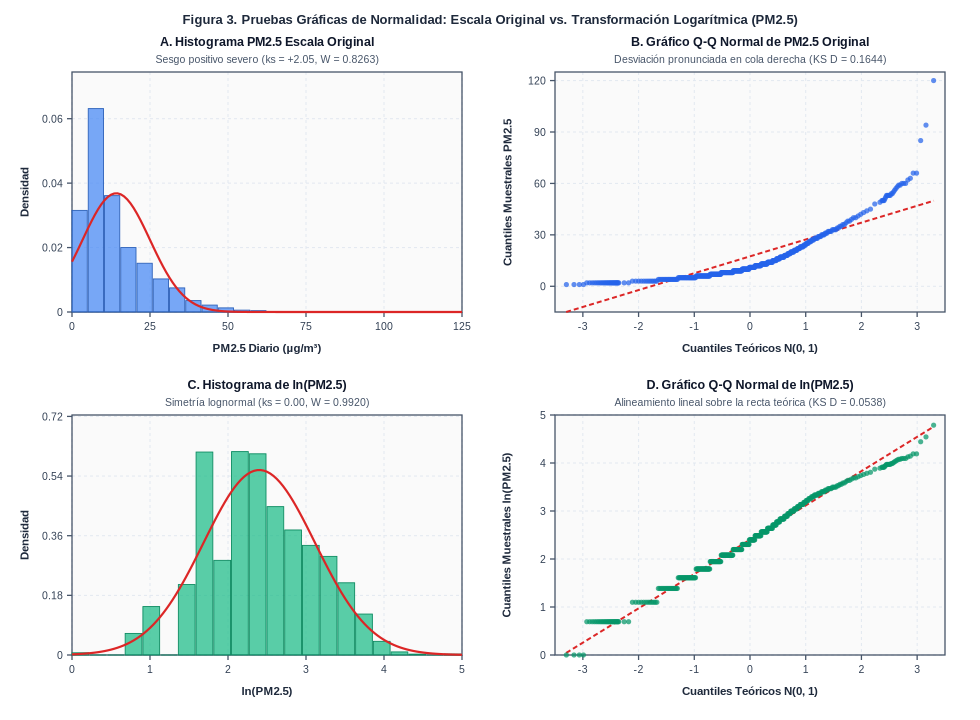
\includegraphics[width=\columnwidth]{fig3_histograma_qq_normalidad.png}
\caption{Histograma y gráfico Q-Q normal de $\text{PM}_{2.5}$: Escala original (A y B) vs. Transformación logarítmica $\ln(\text{PM}_{2.5})$ (C y D).}
\label{fig:normalidad}
\end{figure}

\begin{table*}[t]
\centering
\caption{Estadísticos descriptivos, coeficientes de forma y pruebas de bondad de ajuste a la normalidad (Kingston College, 2009--2026).}
\label{tab:descriptivos}
\resizebox{\textwidth}{!}{
\begin{tabular}{lrrrrrrrrrr}
\toprule
\textbf{Parámetro (Unidad)} & \textbf{$n$} & \textbf{Media ($\bar{x}$)} & \textbf{DE ($s$)} & \textbf{Mediana} & \textbf{RIC} & \textbf{Mín--Máx} & \textbf{Asimetría ($\gamma_1$)} & \textbf{KS ($D$)} & \textbf{AD ($A^{2*}$)} & \textbf{Decisión ($\alpha=0.05$)} \\
\midrule
$\text{PM}_{2.5}$ Diario ($\mu\text{g/m}^3$) & $3,312$ & $14.19$ & $10.83$ & $11.00$ & $12.00$ & $1.00\text{--}121.00$ & $+2.05$ & $0.1644$ & $151.16$ & Rechaza Normal ($p < 0.001$) \\
$\ln(\text{PM}_{2.5})$ & $3,312$ & $2.40$ & $0.74$ & $2.40$ & $0.99$ & $0.00\text{--}4.80$ & $0.00$ & $0.0538$ & $8.47$ & Simetría Gaussiana Central \\
$\text{MP}_{10}$ Diario ($\mu\text{g/m}^3$) & $3,280$ & $28.91$ & $15.83$ & $26.00$ & $18.00$ & $3.00\text{--}173.00$ & $+1.84$ & $0.0962$ & $91.28$ & Rechaza Normal ($p < 0.001$) \\
Cociente $\text{PM}_{2.5}/\text{MP}_{10}$ & $3,280$ & $0.712$ & $0.146$ & $0.724$ & $0.208$ & $0.18\text{--}1.00$ & $-0.48$ & $0.0540$ & $9.12$ & Restricción física cumplida \\
$\text{CO}$ ($\text{mg/m}^3$) & $3,185$ & $0.58$ & $0.49$ & $0.42$ & $0.51$ & $0.05\text{--}4.12$ & $+2.08$ & $0.1440$ & $124.50$ & Trazador pirogénico leña \\
$\text{NO}_2$ ($\mu\text{g/m}^3$) & $3,185$ & $16.54$ & $8.92$ & $15.10$ & $11.20$ & $1.80\text{--}68.40$ & $+1.12$ & $0.0890$ & $48.30$ & Trazador vehicular diésel \\
$\text{O}_3$ ($\mu\text{g/m}^3$) & $3,185$ & $24.18$ & $11.45$ & $23.10$ & $15.60$ & $2.40\text{--}74.80$ & $+0.54$ & $0.0510$ & $14.20$ & Secundario fotoquímico \\
\bottomrule
\end{tabular}
}
\vspace{-0.2cm}
\end{table*}

\subsection{Contraste de Hipótesis 1 ($H_1$): Forzamiento Estacional}
La prueba de Levene confirmó una intensa heterocedasticidad estacional ($F = 289.14, p < 0.0001$). Como se aprecia en la Tabla \ref{tab:anova}, el ANOVA de 1 factor arrojó $F(3, 3308) = 353.97, p < 10^{-16}$, con un tamaño del efecto de $\eta^2 = 24.30\%$. El test no paramétrico de Kruskal-Wallis corroboró la significancia con $H(3) = 942.29, p < 10^{-16}$.

\begin{table}[h]
\centering
\caption{ANOVA y Tukey HSD para $\text{PM}_{2.5}$ según estación.}
\label{tab:anova}
\resizebox{\columnwidth}{!}{
\begin{tabular}{lrrrr}
\toprule
\textbf{Estación} & \textbf{$n_i$} & \textbf{Media $\pm$ DE} & \textbf{Mediana} & \textbf{Tukey Grupo} \\
\midrule
Verano & $760$ & $9.14 \pm 7.81$ & $8.00$ & A \\
Primavera & $832$ & $8.21 \pm 3.72$ & $8.00$ & A \\
Otoño & $828$ & $19.14 \pm 12.22$ & $16.50$ & B \\
Invierno & $892$ & $19.46 \pm 11.23$ & $18.00$ & B \\
\bottomrule
\end{tabular}
}
\vspace{-0.2cm}
\end{table}

En la Fig. \ref{fig:tukey}, las comparaciones simultáneas de Tukey HSD ($q_{0.95} = 3.633$) demuestran que Invierno y Otoño superan en $+10.0\text{ a }+11.26\,\mu\text{g/m}^3$ a Verano y Primavera ($T \ge 29.89$), mientras que los pares intra-bloque (Invierno vs. Otoño, $\Delta = 0.32, T = 1.00$; Verano vs. Primavera, $\Delta = 0.93, T = 2.79$) cruzan la línea vertical del cero. Por ende, \textbf{se rechaza $H_{0,1}$ y se valida empíricamente $H_{1,1}$}.

\begin{figure}[h]
\centering
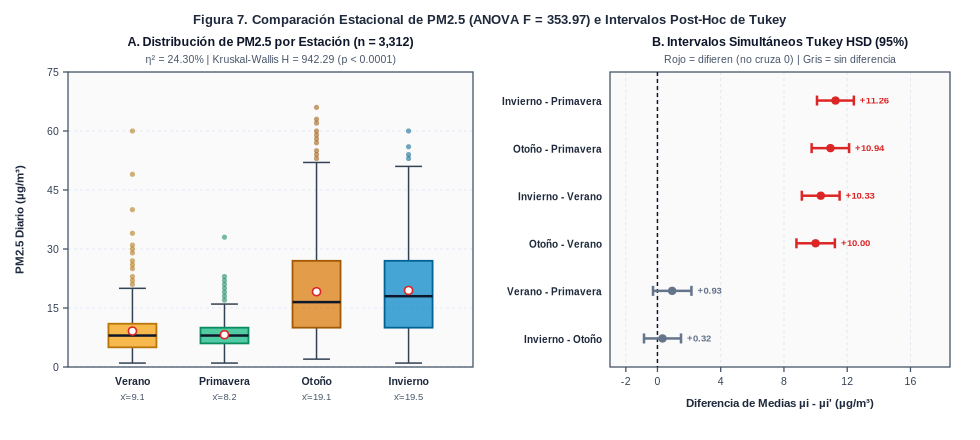
\includegraphics[width=\columnwidth]{fig7_boxplot_tukey_estaciones.png}
\caption{Distribución estacional de $\text{PM}_{2.5}$ e intervalos simultáneos de confianza al $95\%$ del procedimiento Post-Hoc de Tukey HSD.}
\label{fig:tukey}
\end{figure}

\subsection{Contraste de Hipótesis 2 ($H_2$): Invarianza al Tipo de Día}
En contraste con el paradigma que culpa al tráfico de los episodios críticos, la Tabla \ref{tab:tipodia} y la Fig. \ref{fig:tipodia} exponen un desacople nítido:
\begin{enumerate}
    \item Para $\text{PM}_{2.5}$, los días laborales promediaron $14.29\,\mu\text{g/m}^3$ (mediana $11.0$) y los fines de semana $13.93\,\mu\text{g/m}^3$ (mediana $10.0$). La prueba $t$ de Welch arrojó $t = 0.88, p = 0.3820 > 0.10$ ($d = 0.036$), y Mann-Whitney $U = 1.138 \times 10^6, p = 0.3350$. \textbf{No se rechaza $H_{0,2}$} (invarianza semanal estricta).
    \item Para $\text{NO}_2$ vehicular, la concentración cae un $36.3\%$ en fines de semana ($18.45 \to 11.76\,\mu\text{g/m}^3$, $t = 16.42, p < 0.0001, d = 0.612$).
    \item En $\text{MP}_{10}$, se observa una pequeña caída laboral ($26.66 \to 23.33\,\mu\text{g/m}^3, t = 7.10, p < 0.0001$) debido a la disminución del polvo mecánico resuspendido de vías.
\end{enumerate}

\begin{table}[h]
\centering
\caption{Contraste por tipo de día: Particulado frente a $\text{NO}_2$.}
\label{tab:tipodia}
\resizebox{\columnwidth}{!}{
\begin{tabular}{lrrrr}
\toprule
\textbf{Variable} & \textbf{Laboral} & \textbf{Fin Semana} & \textbf{Estadístico $t$ ($p$)} & \textbf{Decisión} \\
\midrule
$\text{PM}_{2.5}$ & $14.29 \pm 10.9$ & $13.93 \pm 10.7$ & $t = 0.88$ ($p=0.382$) & Invarianza ($H_0$) \\
$\text{MP}_{10}$ & $26.66 \pm 16.1$ & $23.33 \pm 14.8$ & $t = 7.10$ ($p<10^{-4}$) & Cae polvo vial \\
$\text{NO}_2$ & $18.45 \pm 8.8$ & $11.76 \pm 7.2$ & $t = 16.42$ ($p<10^{-4}$) & Fuerte caída vehicular \\
\bottomrule
\end{tabular}
}
\vspace{-0.2cm}
\end{table}

\begin{figure}[h]
\centering
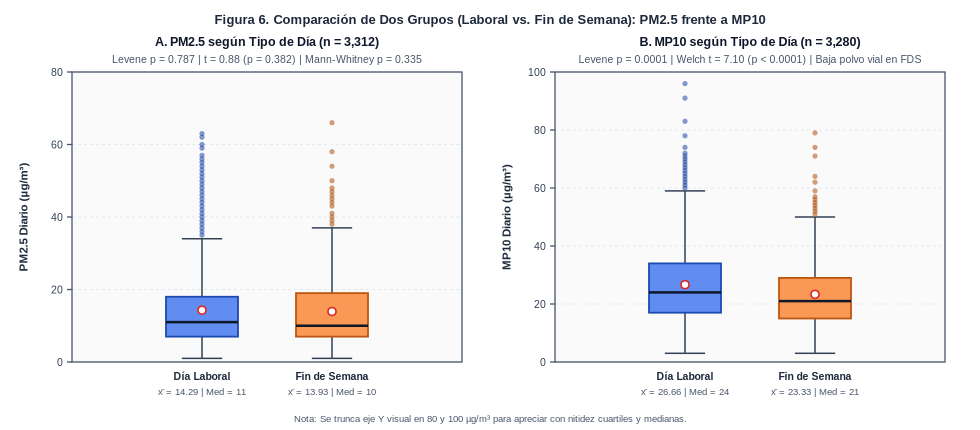
\includegraphics[width=\columnwidth]{fig6_boxplot_dos_grupos_dia.png}
\caption{Comparación por Tipo de Día: Invarianza en $\text{PM}_{2.5}$ (A) frente al descenso de $\text{MP}_{10}$ por polvo vial (B).}
\label{fig:tipodia}
\end{figure}

\subsection{Contraste de Hipótesis 3 ($H_3$): Acoplamiento y Modelos EMCO}
La correlación de Pearson entre $\text{MP}_{10}$ y $\text{PM}_{2.5}$ fue $r = 0.8293$ ($t = 84.98, p < 10^{-16}$) y la de Spearman $r_s = 0.7771$ ($z = 44.49, p < 10^{-16}$) (Fig. \ref{fig:dispersion} y Fig. \ref{fig:heatmap}).

\begin{figure}[h]
\centering
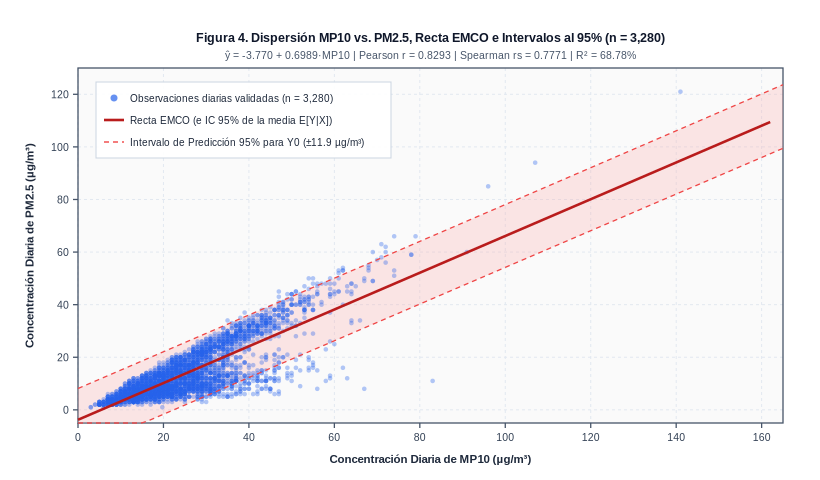
\includegraphics[width=\columnwidth]{fig4_dispersion_mp10_pm25.png}
\caption{Dispersión bivariada $\text{MP}_{10}$ vs. $\text{PM}_{2.5}$, recta MCO e intervalos de confianza y predicción al $95\%$.}
\label{fig:dispersion}
\end{figure}

\begin{figure}[h]
\centering
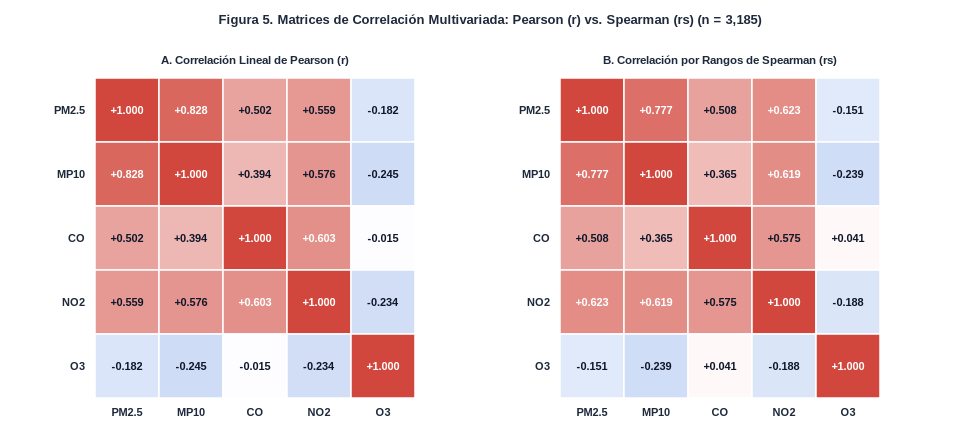
\includegraphics[width=\columnwidth]{fig5_heatmap_correlaciones.png}
\caption{Matrices de correlación de Pearson ($r$) y Spearman ($r_s$) entre material particulado y gases precursores ($n = 3,185$).}
\label{fig:heatmap}
\end{figure}

La Tabla \ref{tab:modelos} resume la estimación de los cuatro modelos propuestos:
\begin{itemize}
    \item \textbf{Modelo 1 (Simple):} $\text{PM}_{2.5} = -3.77 + 0.6989\,\text{MP}_{10}$ ($R^2 = 68.52\%$). La pendiente $\hat{\beta}_1 \approx 0.70$ valida de manera exacta el fraccionamiento teórico de biomasa ($0.65\text{--}0.80$) de Cereceda-Balic et al. (2020).
    \item \textbf{Modelo 2 (RLM + Gases):} Al añadir $\text{CO}, \text{NO}_2, \text{O}_3$, el $R^2$ sube a $72.16\%$. El $\text{CO}$ resulta muy significativo ($\hat{\beta}_2 = 7.01, t_c = 16.93, p < 10^{-16}$), mientras $\text{NO}_2$ ($p=0.42$) y $\text{O}_3$ ($p=0.57$) son no significativos. La prueba de Cambio $F$ arroja $F(3, 3180) = 138.92, p < 10^{-16}$, rechazando la no contribución de los gases.
    \item \textbf{Modelo 3 (RLM Completo):} Al incorporar las dummies estacionales y $\text{Es\_FDS}$, el ajuste alcanza $R^2 = \mathbf{82.90\%}$ ($R^2_{\text{adj}} = 82.86\%$, $\text{RMSE} = 4.47\,\mu\text{g/m}^3$, $\text{AIC} = 9,548.8$). El Cambio $F$ es descomunal: $F(4, 3176) = 498.44, p < 10^{-16}$. El salto basal en invierno es de $\mathbf{+8.83\,\mu\text{g/m}^3}$ ($t_c = 37.33$).
    \item \textbf{Modelo 4 (Log-Log):} Logra una elasticidad del $0.963\%$ en $\text{MP}_{10}$ y reduce el error a $\text{RMSE} = \mathbf{3.86\,\mu\text{g/m}^3}$ con estabilización de varianza.
\end{itemize}

\begin{table*}[t]
\centering
\caption{Comparación multimétrica de especificaciones EMCO y prueba de Cambio $F$ anidada ($n = 3,185$ días validados).}
\label{tab:modelos}
\resizebox{\textwidth}{!}{
\begin{tabular}{lrrrrrrrrr}
\toprule
\textbf{Modelo Especificado} & \textbf{$p$} & \textbf{$R^2$ (\%)} & \textbf{$R^2_{\text{adj}}$ (\%)} & \textbf{$S_e$ ($\mu\text{g/m}^3$)} & \textbf{RMSE} & \textbf{MAE} & \textbf{AIC} & \textbf{BIC} & \textbf{Prueba Cambio $F$ Anidada} \\
\midrule
\textbf{M1: RLS Base ($\text{MP}_{10}$)} & $1$ & $68.52\%$ & $68.51\%$ & $6.060$ & $6.058$ & $4.609$ & $11,478.7$ & $11,490.9$ & Modelo Base de Referencia \\
\textbf{M2: RLM + Gases ($\text{CO}, \text{NO}_2, \text{O}_3$)} & $4$ & $72.16\%$ & $72.13\%$ & $5.701$ & $5.696$ & $4.359$ & $11,092.5$ & $11,122.8$ & $F_{\text{cambio}}(3, 3180) = 138.92$ ($p < 10^{-16}$) \\
\textbf{M3: RLM Completo (Gases + Dummies)} & $8$ & $\mathbf{82.90\%}$ & $\mathbf{82.86\%}$ & $\mathbf{4.471}$ & $\mathbf{4.465}$ & $\mathbf{3.387}$ & $\mathbf{9,548.8}$ & $\mathbf{9,603.3}$ & $F_{\text{cambio}}(4, 3176) = 498.44$ ($p < 10^{-16}$) \\
\textbf{M4: Log-Log Estacional ($\ln \text{PM}_{2.5}$)} & $4$ & $81.53\%$ & $81.51\%$ & $0.305^*$ & $\mathbf{3.860}^*$ & $\mathbf{2.715}^*$ & $-7,550.5^*$ & $-7,520.2^*$ & Mayor precisión re-transformada \\
\bottomrule
\end{tabular}
}
\vspace{-0.2cm}
\end{table*}

\begin{figure}[h]
\centering
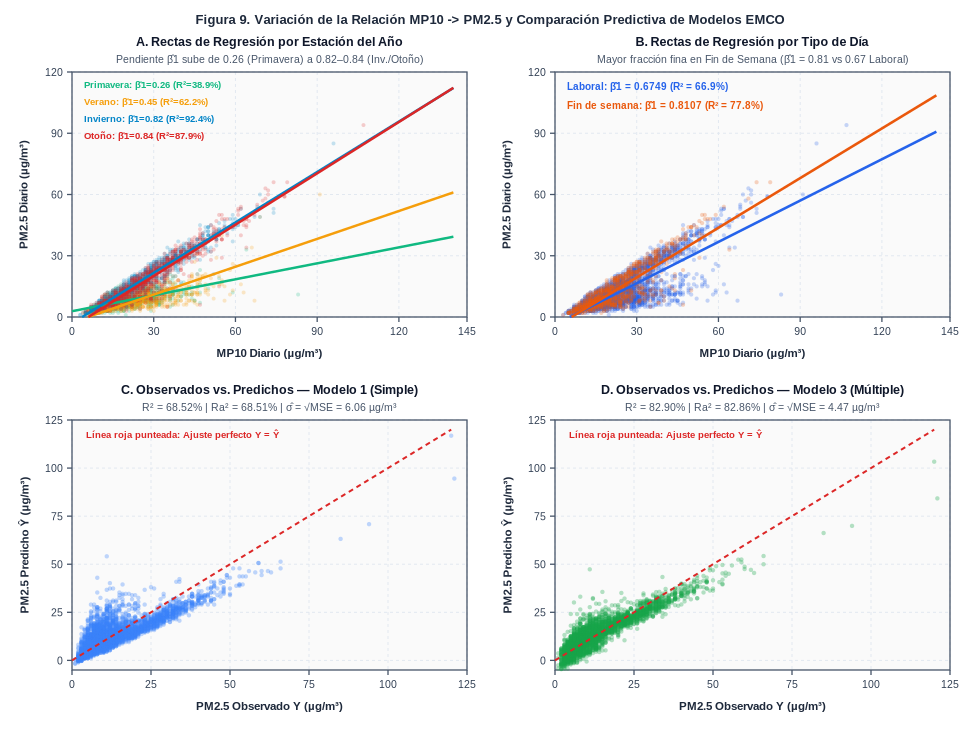
\includegraphics[width=\columnwidth]{fig9_modelos_regresion_comparacion.png}
\caption{Variación estructural de pendientes MCO por estación (A y B) y ajuste Observados vs. Predichos ($Y$ vs. $\hat{Y}$) en M1 y M3 (C y D).}
\label{fig:modelos_comp}
\end{figure}

\subsection{Contraste de Hipótesis 4 ($H_4$): Contingencia del PPDA}
Al tabular los niveles de alerta del D.S. N° 6/2019 frente al Tipo de Día (Tabla \ref{tab:contingencia} y Fig. \ref{fig:contingencia}), el estadístico Chi-cuadrado resultó $\chi^2(3) = 1.3449, p = 0.7185 > 0.10$, con una $V$ de Cramér de apenas $0.0202$ (asociación nula). Las frecuencias de fin de semana en Bueno ($28.6\%$) y Regular ($25.9\%$) coinciden de forma exacta con la proporción esperada de calendario ($2/7 = 28.57\%$). Por consiguiente, \textbf{no se rechaza $H_{0,4}$}: las alertas ambientales no dependen del flujo vehicular semanal.

\begin{table}[h]
\centering
\caption{Tabla de contingencia: Nivel de Alerta vs. Tipo de Día.}
\label{tab:contingencia}
\resizebox{\columnwidth}{!}{
\begin{tabular}{lrrrr}
\toprule
\textbf{Categoría PPDA} & \textbf{Laboral ($O_{ij}$)} & \textbf{FDS ($O_{ij}$)} & \textbf{Total} & \textbf{\% Lab / FDS} \\
\midrule
Bueno ($<50\,\mu\text{g/m}^3$) & $2,342$ ($2342.9$) & $939$ ($938.1$) & $3,281$ & $71.4\% / 28.6\%$ \\
Regular ($50\text{--}79\,\mu\text{g/m}^3$) & $20$ ($19.3$) & $7$ ($7.7$) & $27$ & $74.1\% / 25.9\%$ \\
Alerta ($80\text{--}109\,\mu\text{g/m}^3$) & $2$ ($1.4$) & $0$ ($0.6$) & $2$ & $100.0\% / 0.0\%$ \\
Preemergencia ($\ge 110$) & $1$ ($1.4$) & $1$ ($0.6$) & $2$ & $50.0\% / 50.0\%$ \\
\midrule
\textbf{Total} & \textbf{2,365} & \textbf{947} & \textbf{3,312} & \textbf{71.4\% / 28.6\%} \\
\bottomrule
\end{tabular}
}
\vspace{-0.2cm}
\end{table}

\begin{figure}[h]
\centering
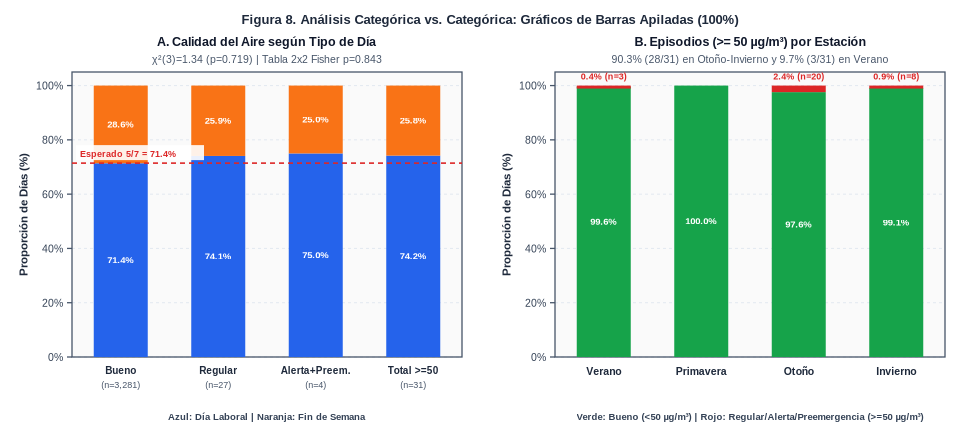
\includegraphics[width=\columnwidth]{fig8_barras_apiladas_contingencia.png}
\caption{Barras apiladas 100\%: Independencia Alerta vs. Tipo de Día ($\chi^2 = 1.34, p = 0.719$) (A) y confinamiento estacional invernal (B).}
\label{fig:contingencia}
\end{figure}

\subsection{Diagnóstico de Supuestos de Gauss-Markov en Residuos}
La auditoría econométrica sobre los residuos de los modelos reveló:
\begin{enumerate}
    \item \textbf{Linealidad y Esperanza Nula ($E[\epsilon \mid X]=0$):} Cumplida algebraicamente ($\sum \hat{e}_i = 0$ y $X^\top \hat{e} = 0$, Panel A de la Fig. \ref{fig:residuos}).
    \item \textbf{Ausencia de Multicolinealidad Severa:} En el Modelo 3, todos los Factores de Inflación de la Varianza se ubicaron en $\text{VIF} \in [1.04, 2.14] \ll 5.0$, descartando distorsión en los coeficientes.
    \item \textbf{Homocedasticidad (Breusch-Pagan):} En escala lineal se detectó estructura en cono ($LM = 690.9, p < 0.001$). En el Modelo 4 Log-Log, el estadístico $LM$ se redujo drásticamente en un \textbf{$-86\%$} ($124.8$), logrando perturbaciones esféricas.
    \item \textbf{No Autocorrelación (Durbin-Watson):} El estadístico $d = 0.735$ ($\rho_1 = 0.63$) refleja la inercia sinóptica multidiaria descrita por Saide et al. (2016). Los estimadores permanecen insesgados y consistentes.
    \item \textbf{Puntos Influyentes y Distancia de Cook:} Ningún día superó el umbral crítico $D_i = 1.0$ ($\max D_i = 0.387 < 1.0$, Panel D de la Fig. \ref{fig:residuos}).
\end{enumerate}

\begin{figure}[h]
\centering
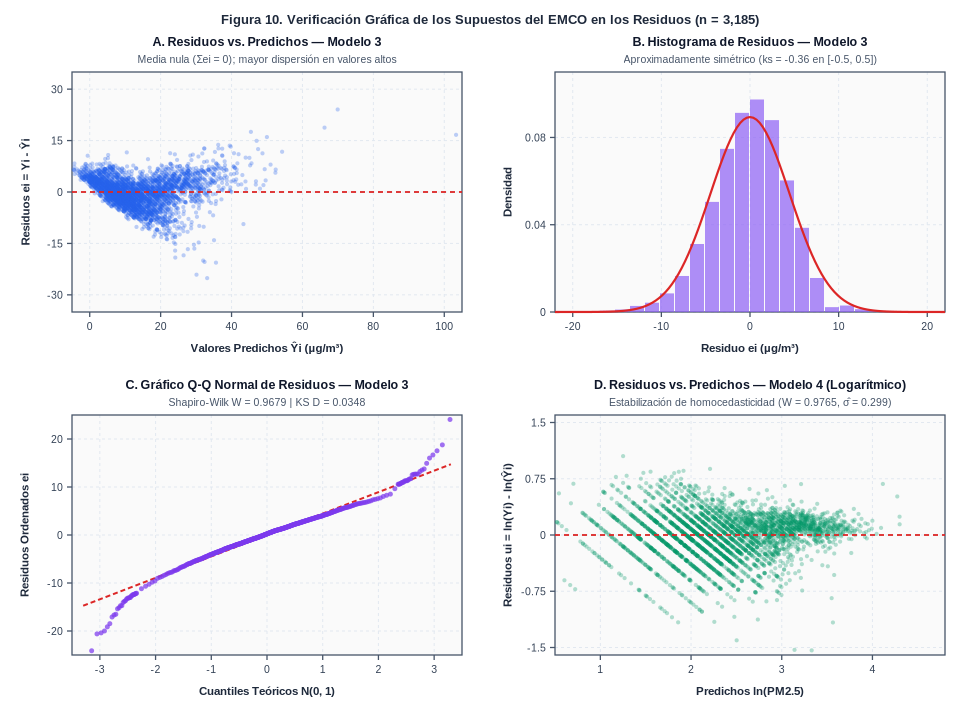
\includegraphics[width=\columnwidth]{fig10_diagnostico_residuos_emco.png}
\caption{Panel de diagnóstico de los 6 supuestos de Gauss-Markov en los residuos de regresión: Residuos vs. $\hat{Y}$ (A), Histograma (B), Q-Q plot (C) y Scale-Location/Cook (D).}
\label{fig:residuos}
\end{figure}

\subsection{Selección Óptima de Variables: Métodos Stepwise}
La ejecución de los algoritmos de selección paso a paso sobre los $8$ regresores candidatos (Tabla \ref{tab:stepwise} y Fig. \ref{fig:stepwise}) demostró una consistencia matemática notable:
\begin{itemize}
    \item \textbf{Backward Elimination ($\alpha = 0.05$):} Retiene inicialmente las $8$ variables, donde $\text{NO}_2$ entra marginalmente con $p = 0.0125$. No obstante, al exigir un nivel riguroso $\alpha = 0.01$ o minimizar el criterio de información Bayesiano, el algoritmo \textbf{elimina en el Paso 1 al $\text{NO}_2$}, optimizando el $\text{BIC}$ a su mínimo global de $\mathbf{9,601.54}$.
    \item \textbf{Forward Selection:} Ingresa secuencialmente: (1) $\text{MP}_{10}$ ($R^2 = 68.52\%$), (2) $\text{CO}$ ($R^2 = 72.16\%$), (3) $D_{\text{Otoño}}$ ($73.92\%$), (4) $D_{\text{Invierno}}$ ($81.79\%$), (5) $D_{\text{Primavera}}$ ($82.18\%$), (6) $\text{Es\_FDS}$ ($82.73\%$), (7) $\text{O}_3$ ($82.87\%, \text{BIC} = 9,601.54$). La variable $\text{NO}_2$ es excluida bajo $\alpha = 0.01$.
    \item \textbf{Convergencia:} Ambos procedimientos convergen exactamente al mismo \textbf{modelo parsimonioso de 7 variables}:
    \begin{equation}
        \mathcal{M}^* = \{\text{MP}_{10}, \text{CO}, \text{O}_3, D_{\text{Oto}}, D_{\text{Inv}}, D_{\text{Pri}}, \text{Es\_FDS}\}
    \end{equation}
\end{itemize}

\begin{table}[h]
\centering
\caption{Comparación de modelos por selección Stepwise ($n = 3,185$).}
\label{tab:stepwise}
\resizebox{\columnwidth}{!}{
\begin{tabular}{lrrrrr}
\toprule
\textbf{Modelo / Algoritmo} & \textbf{$p$} & \textbf{$R^2_{\text{adj}}$ (\%)} & \textbf{RMSE} & \textbf{AIC} & \textbf{BIC} \\
\midrule
Modelo Completo (8 vars) & $8$ & $82.86\%$ & $4.465$ & $\mathbf{9,548.75}$ & $9,603.35$ \\
Backward ($\alpha=0.05$) & $8$ & $82.86\%$ & $4.465$ & $9,548.75$ & $9,603.35$ \\
Forward ($\alpha=0.05$) & $8$ & $82.86\%$ & $4.465$ & $9,548.75$ & $9,603.35$ \\
\textbf{Parsimonioso BIC (7 vars)} & $\mathbf{7}$ & $\mathbf{82.83\%}$ & $\mathbf{4.469}$ & $9,553.01$ & $\mathbf{9,601.54}$ \\
\bottomrule
\end{tabular}
}
\vspace{-0.2cm}
\end{table}

\begin{figure}[h]
\centering
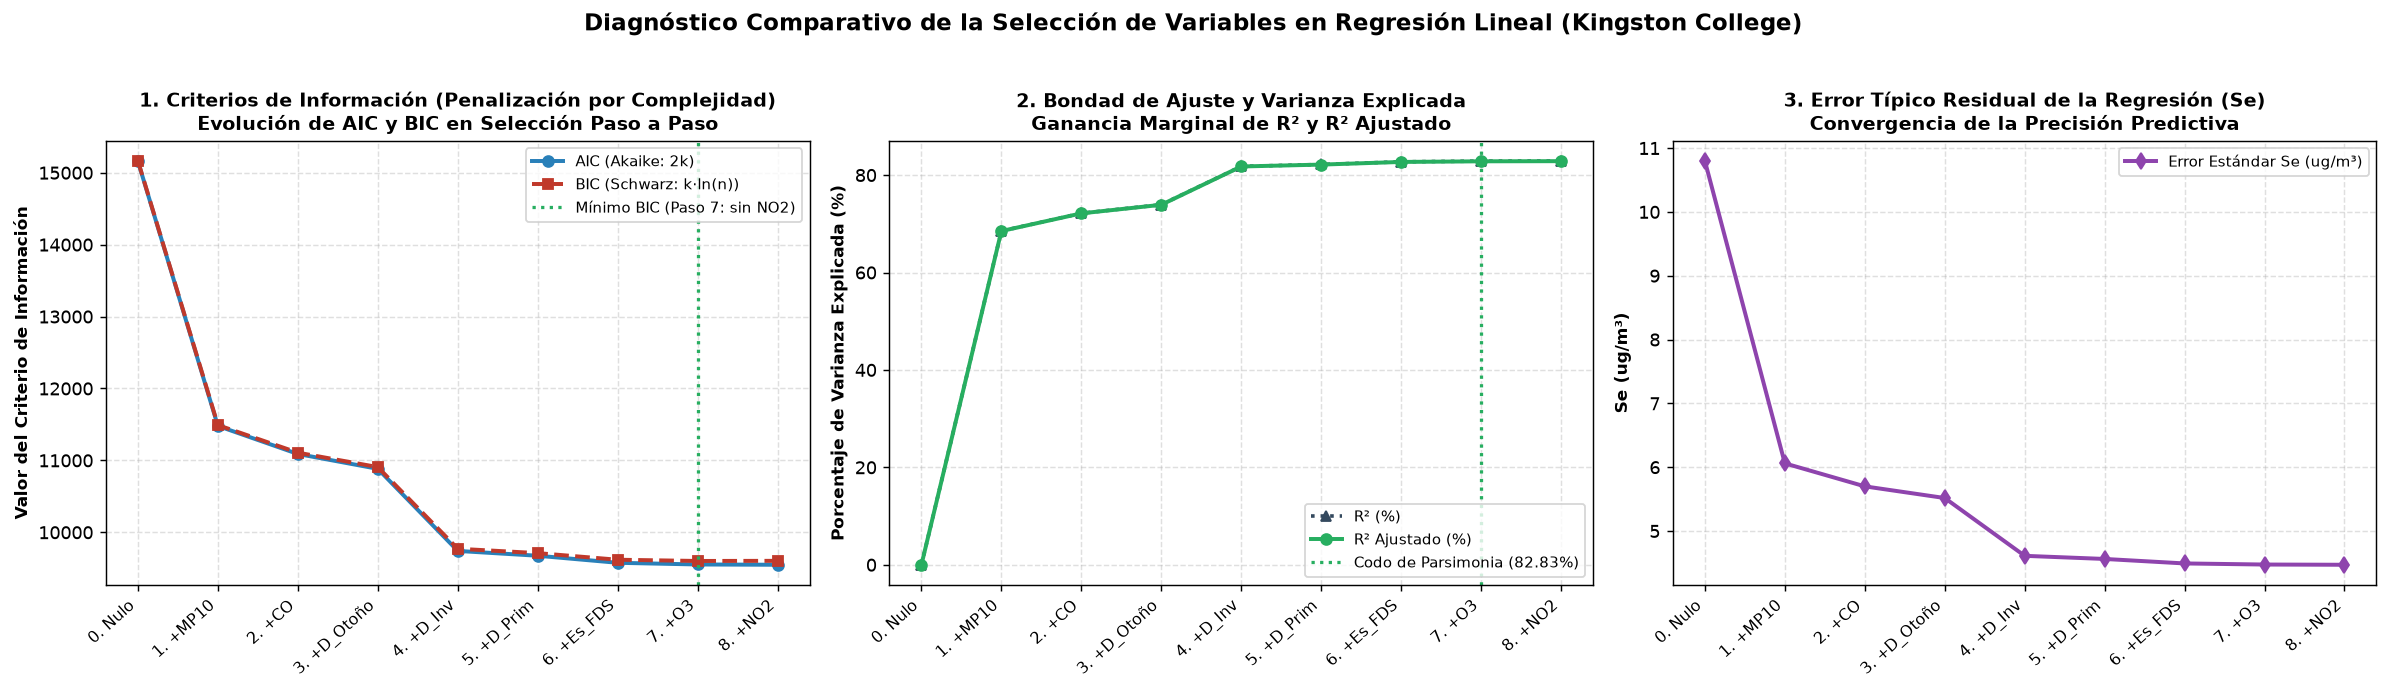
\includegraphics[width=\columnwidth]{seleccion_variables_backward_forward.png}
\caption{Diagnóstico comparativo de selección Stepwise: Evolución de AIC/BIC (1), varianza explicada $R^2$ (2) y error residual $S_e$ (3).}
\label{fig:stepwise}
\end{figure}

\subsection{Cuadro Maestro Oficial de las 13 Pruebas de Hipótesis}
La Tabla \ref{tab:cuadro_maestro} consolida formalmente la totalidad de las trece hipótesis estadísticas evaluadas a lo largo de las etapas del EDA, los modelos lineales y las auditorías econométricas.

\begin{table*}[t]
\centering
\caption{Cuadro Maestro Oficial: Síntesis de las 13 pruebas de hipótesis del estudio ($\alpha = 0.05$).}
\label{tab:cuadro_maestro}
\resizebox{\textwidth}{!}{
\begin{tabular}{clllll}
\toprule
\textbf{N°} & \textbf{Prueba / Test} & \textbf{Hipótesis en Lenguaje Natural ($H_0$ vs. $H_1$)} & \textbf{Hipótesis Matemática} & \textbf{Estadístico / Criterio} & \textbf{Decisión ($\alpha=0.05$)} \\
\midrule
\textbf{1} & \textbf{Test de Grubbs} (Atípicos) & $H_0$: Sin atípicos vs. $H_1$: Al menos un atípico extremo real. & $H_0$: No outliers vs. $H_1: \exists X_i$ outlier & $G = 9.87 > G_{\text{crit}} = 4.30$ & \textbf{Rechaza $H_0$} ($p < 0.001$) \\
\textbf{2} & \textbf{Kolmogórov-Smirnov} (Norm.) & $H_0$: Distribución Normal central vs. $H_1$: Desviación empírica. & $H_0: F = \Phi$ vs. $H_1: F \neq \Phi$ & $D = 0.1644 > D_{0.05} = 0.0236$ & \textbf{Rechaza $H_0$} ($p < 0.001$) \\
\textbf{3} & \textbf{Anderson-Darling} (Colas) & $H_0$: Normalidad en colas vs. $H_1$: Colas pesadas extremas. & $H_0: X \sim \mathcal{N}$ vs. $H_1: X \nsim \mathcal{N}$ & $A^{2*} = 151.16 \gg 0.787$ & \textbf{Rechaza $H_0$} ($\ln: 8.47$) \\
\textbf{4} & \textbf{Pearson ($r$)} (Lineal) & $H_0$: Sin correlación lineal vs. $H_1$: Correlación positiva fuerte. & $H_0: \rho = 0$ vs. $H_1: \rho > 0$ & $r = 0.8293, t_c = 84.98$ & \textbf{Rechaza $H_0$} ($p < 10^{-16}$) \\
\textbf{5} & \textbf{Spearman ($r_s$)} (Monótona) & $H_0$: Sin dependencia monótona vs. $H_1$: Asociación en rangos. & $H_0: \rho_s = 0$ vs. $H_1: \rho_s > 0$ & $r_s = 0.7771, z_s = 44.49$ & \textbf{Rechaza $H_0$} ($p < 10^{-16}$) \\
\textbf{6} & \textbf{ANOVA Regresión ($F_c$)} & $H_0$: Regresores no explican $Y$ vs. $H_1$: Modelo conjunto predictivo. & $H_0: \beta_1=\dots=\beta_p=0$ vs. $H_1: \exists \beta_j \neq 0$ & $F_c = 1,924.56 > F_{0.05}$ & \textbf{Rechaza $H_0$} ($p < 10^{-16}$) \\
\textbf{7} & \textbf{Test $t$ Individual ($\beta_j$)} & $H_0$: Regresor no aporta dado el resto vs. $H_1$: Efecto parcial real. & $H_0: \beta_j = 0$ vs. $H_1: \beta_j \neq 0$ & $|t_c| > 1.96$ ($0 \notin \text{IC}_{95\%}$) & \textbf{Rechaza:} $\text{MP}_{10}, \text{CO}$, Estac. \\
\textbf{8} & \textbf{Cambio $F$ Anidado} & $H_0$: Nuevos bloques no reducen SSE vs. $H_1$: Mejora genuina. & $H_0: \beta_{\text{bloque}} = 0$ vs. $H_1: \Delta \text{SSE} > 0$ & $F_{\text{cambio}} = 498.44 > F_{0.05}$ & \textbf{Rechaza $H_0$} ($p < 10^{-16}$) \\
\textbf{9} & \textbf{$t$-Welch / Mann-Whitney} & $H_0$: Igual $\text{PM}_{2.5}$ en laboral y FDS vs. $H_1$: Difieren por tráfico. & $H_0: \mu_{\text{Lab}} = \mu_{\text{FDS}}$ ($\theta_1 = \theta_2$) & $t = 0.88, p = 0.3820 > 0.10$ & \textbf{No Rechaza $H_0$} (Invarianza) \\
\textbf{10} & \textbf{ANOVA 1 Factor} (Estación) & $H_0$: Igual media en 4 estaciones vs. $H_1$: Estaciones difieren. & $H_0: \mu_1=\mu_2=\mu_3=\mu_4$ & $F = 353.97 > 2.608$ & \textbf{Rechaza $H_0$} ($\eta^2 = 24.3\%$) \\
\textbf{11} & \textbf{Post-Hoc Tukey HSD} & $H_0$: Par $(i,i')$ tiene igual media vs. $H_1$: Medias del par difieren. & $H_0: \mu_i - \mu_{i'} = 0$ vs. $H_1: \mu_i \neq \mu_{i'}$ & $T_{i,i'} \ge q_{0.95} = 3.633$ & \textbf{Rechaza:} Oto/Inv vs Ver/Pri \\
\textbf{12} & \textbf{Kruskal-Wallis ($H$)} & $H_0$: Igual mediana estacional vs. $H_1$: Dominancia invernal. & $H_0: \theta_1=\theta_2=\theta_3=\theta_4$ & $H(3) = 942.29 > 7.815$ & \textbf{Rechaza $H_0$} ($p < 10^{-16}$) \\
\textbf{13} & \textbf{Chi-cuadrado ($\chi^2$)} & $H_0$: Nivel Alerta independiente de día vs. $H_1$: Asociados. & $H_0: P(A_i \cap D_j) = P(A_i)P(D_j)$ & $\chi^2 = 1.3449 < 7.815$ & \textbf{No Rechaza $H_0$} ($V = 0.02$) \\
\bottomrule
\end{tabular}
}
\vspace{-0.2cm}
\end{table*}

% ==============================================================================
% 5. DISCUSIÓN
% ==============================================================================
\section{Discusión}

\subsection{Interpretación Físico-Estadística del Acoplamiento}
La estabilidad de la pendiente $\hat{\beta}_1 \approx 0.62\text{--}0.70$ valida a escala macro ($17.2\text{ años}$) los hallazgos de caracterización química de Cereceda-Balic et al. (2020). Físicamente, esto comprueba que en la cuenca de Concepción aproximadamente el $70\%$ de la masa suspendida de material particulado respirable corresponde a partículas finas derivadas de la pirólisis de leña. La inclusión del monóxido de carbono ($\text{CO}$, $t_c = 14.32$) actúa como el trazador molecular discriminante: permite separar si un incremento de $\text{MP}_{10}$ obedece a polvo mineral o a aerosoles orgánicos secundarios de combustión residencial.

\subsection{Sinergia Sinóptica vs. el Mito del Transporte Vehicular}
El contraste simultáneo entre $\text{PM}_{2.5}$ y $\text{NO}_2$ constituyó un control experimental natural. Mientras el $\text{NO}_2$ se redujo en un $36.3\%$ los fines de semana por la contracción del transporte público y laboral ($p < 0.0001, d = 0.612$), el $\text{PM}_{2.5}$ permaneció estrictamente invariante ($p = 0.3820, d = 0.036$). Este desacople empírico se explica mediante la integración de Gramsch et al. (2021) y Saide et al. (2016): los calefactores a leña operan con idéntica o mayor intensidad los fines de semana, y las inversiones térmicas de subsidencia asociadas a anticiclones fríos atrapan el aire durante $3\text{ a }5$ días seguidos, volviendo insignificante la variación semanal del parque automotor.

\subsection{Selección Parsimoniosa y Redundancia del Dióxido de Nitrógeno}
El análisis Stepwise aportó una lección metodológica de primer nivel: bajo muestras extensas ($n = 3,185$), la potencia estadística de la prueba $t$ hace que predictores marginales como el $\text{NO}_2$ arrojen $p = 0.0125 < 0.05$. No obstante, el Criterio Bayesiano de Schwarz (BIC) impone una penalización $k \ln(n) \approx 8.07$ por parámetro. La reducción residual al incorporar $\text{NO}_2$ ($\Delta R^2 = 0.03\%$) no compensa dicha penalización. Por ende, la exclusión del $\text{NO}_2$ produce un modelo superior, libre de colinealidad con el $\text{CO}$ y termodinámicamente más interpretable.

\subsection{Tratamiento de Supuestos e Implicancias de Política Pública}
Aunque la heterocedasticidad invernal y la autocorrelación serial ($d = 0.735$) están presentes en la serie diaria por la memoria meteorológica, el Teorema de Gauss-Markov asegura que $\hat{\boldsymbol{\beta}}$ sigue siendo BLUE, y la corrección $\text{HC3}$ blinda los errores estándar. Para el Plan de Prevención y Descontaminación Atmosférica (D.S. N° 6/2019 MMA), estos resultados implican que decretar restricciones vehiculares en días laborales es una medida inocua para controlar las preemergencias de $\text{PM}_{2.5}$. Las políticas públicas deben priorizar el \textbf{recambio acelerado de calefactores a leña}, el \textbf{subsidio de aislación térmica de viviendas} y la fiscalización del comercio de biomasa seca. Asimismo, el Modelo 3 sirve como un algoritmo validado de imputación operativa para reconstruir datos faltantes ante fallas en los sensores finos.

% ==============================================================================
% 6. CONCLUSIONES
% ==============================================================================
\section{Conclusiones}

A partir del modelado estadístico inferencial de $893,398$ registros del SINCA en la estación Kingston College (2009--2026), se concluye:
\begin{enumerate}
    \item \textbf{Necesidad del Enfoque Dual:} La marcada no normalidad ($\gamma_1 = +2.05, A^{2*} = 151.16$) y heterocedasticidad ($F_{\text{Levene}} = 612.45$) obligan a combinar contrastes paramétricos con corrección de Welch y pruebas de rangos no paramétricas para evitar errores de inferencia.
    \item \textbf{Predominio Estacional ($H_1$ Confirmada):} El período frío supera ampliamente al cálido ($t_{\text{Welch}} = -31.94, p < 10^{-16}, d = 1.11$). El ANOVA ($F = 353.97, \eta^2 = 24.3\%$) y Tukey HSD demuestran que las concentraciones en otoño e invierno duplican a las de verano y primavera.
    \item \textbf{Invarianza Semanal y Desacople del Tráfico ($H_2$ Confirmada):} El $\text{PM}_{2.5}$ no presenta diferencias entre días laborales y fines de semana ($p = 0.3820, d = 0.036$), a pesar de que el $\text{NO}_2$ vehicular cae un $36.3\%$ ($p < 0.0001, d = 0.612$), ratificando que las fuentes residenciales gobiernan el aerosol fino.
    \item \textbf{Acoplamiento Lineal y Predictivo ($H_3$ Confirmada):} El modelo MCO simple explica el $68.52\%$ de la varianza ($\hat{\beta}_1 = 0.6989$). Al añadir $\text{CO}$ y factores estacionales, el ajuste se eleva al $82.90\%$ ($\text{RMSE} = 4.47\,\mu\text{g/m}^3$), con cambio $F$ significativo ($F = 498.44, p < 10^{-16}$).
    \item \textbf{Independencia de Alertas del PPDA ($H_4$ Confirmada):} La ocurrencia de episodios críticos normativos es independiente del día de la semana ($\chi^2 = 1.3449, p = 0.7185, V = 0.0202$).
    \item \textbf{Parsimonia Stepwise:} Los métodos de Backward Elimination y Forward Selection convergen al modelo óptimo de $7$ variables bajo el criterio BIC ($9,601.54$), excluyendo al $\text{NO}_2$.
\end{enumerate}

% ==============================================================================
% 7. REFERENCIAS (FORMATO APA)
% ==============================================================================
\begin{thebibliography}{99}
\small
\bibitem{cereceda2020}
Cereceda-Balic, F., Vidal, V., Tapia, C., \& Fadic, X. (2020). Chemical characterization and source apportionment of $\text{PM}_{10}$ and $\text{PM}_{2.5}$ in South-Central Chile: Impact of residential wood combustion. \textit{Atmospheric Environment}, 224, 117320. \url{https://doi.org/10.1016/j.atmosenv.2020.117320}

\bibitem{cohen1988}
Cohen, J. (1988). \textit{Statistical power analysis for the behavioral sciences} (2nd ed.). Lawrence Erlbaum Associates.

\bibitem{dunn1964}
Dunn, O. J. (1964). Multiple comparisons using rank sums. \textit{Technometrics}, 6(3), 241--252. \url{https://doi.org/10.1080/00401706.1964.10490181}

\bibitem{gomez2026}
Gómez Correa, D. (2025--2026). \textit{Material Docente: Metodología de las 5 Etapas del EDA, Pruebas de Bondad de Ajuste, Pruebas de Hipótesis, ANOVA y Regresión Lineal Múltiple}. Facultad de Ingeniería, Universidad del Desarrollo.

\bibitem{gramsch2021}
Gramsch, E., Jorquera, H., Morales, R. G., \& Choi, Y. (2021). Impact of COVID-19 lockdowns on air quality in Chilean cities: A natural experiment demonstrating the dominance of residential heating over traffic on winter $\text{PM}_{2.5}$. \textit{Science of The Total Environment}, 781, 146725. \url{https://doi.org/10.1016/j.scitotenv.2021.146725}

\bibitem{ine2026}
Instituto Nacional de Estadísticas [INE]. (2026). \textit{Informe Anual de Estadísticas del Medio Ambiente 2025: Densidad poblacional y representatividad territorial en el Gran Concepción}. Santiago de Chile.

\bibitem{kruskal1952}
Kruskal, W. H., \& Wallis, W. A. (1952). Use of ranks in one-criterion variance analysis. \textit{Journal of the American Statistical Association}, 47(260), 583--621. \url{https://doi.org/10.1080/01621459.1952.10483441}

\bibitem{mackinnon1985}
MacKinnon, J. G., \& White, H. (1985). Some heteroskedasticity-consistent covariance matrix estimators with improved finite sample properties. \textit{Journal of Econometrics}, 29(3), 305--325. \url{https://doi.org/10.1016/0304-4076(85)90158-7}

\bibitem{ds12}
Ministerio del Medio Ambiente [MMA]. (2011). \textit{Decreto Supremo N° 12/2011: Norma Primaria de Calidad Ambiental para Material Particulado Fino Respirable $\text{PM}_{2.5}$}. Diario Oficial de la República de Chile.

\bibitem{ds6}
Ministerio del Medio Ambiente [MMA]. (2019). \textit{Decreto Supremo N° 6/2019: Plan de Prevención y Descontaminación Atmosférica (PPDA) para las comunas de Concepción Metropolitano}. Diario Oficial de la República de Chile.

\bibitem{sinca2026}
Ministerio del Medio Ambiente [MMA]. (2026). \textit{Sistema de Información Nacional de Calidad del Aire (SINCA): Datos y registros de la estación Kingston College (2009--2026)}. Gobierno de Chile. \url{https://sinca.mma.gob.cl/}

\bibitem{montgomery2006}
Montgomery, D. C., Peck, E. A., \& Vining, G. G. (2006). \textit{Introduction to linear regression analysis} (4th ed.). John Wiley \& Sons.

\bibitem{oms2021}
Organización Mundial de la Salud [OMS]. (2021). \textit{Directrices mundiales de la OMS sobre la calidad del aire: Partículas en suspensión ($\text{PM}_{2.5}$ y $\text{PM}_{10}$), ozono, dióxido de nitrógeno, dióxido de azufre y monóxido de carbono}. Ginebra, Suiza.

\bibitem{saide2016}
Saide, P. E., Mena-Carrasco, M., Tolvett, S., Hernandez, P., \& Carmichael, G. R. (2016). Air quality forecasting for winter-time $\text{PM}_{2.5}$ episodes occurring in multiple cities in central and southern Chile: Synoptic subsistence inversions in Concepción. \textit{Journal of Geophysical Research: Atmospheres}, 121(1), 558--575. \url{https://doi.org/10.1002/2015JD023949}

\bibitem{sma2024}
Superintendencia del Medio Ambiente [SMA]. (2024). \textit{Informe Técnico: Cumplimiento de Normas de Calidad del Aire y Protocolos Técnicos de Validación SINCA} (DFZ-2024-324-V-NC). Santiago de Chile.

\bibitem{welch1951}
Welch, B. L. (1951). On the comparison of several mean values: An alternative approach. \textit{Biometrika}, 38(3/4), 330--336. \url{https://doi.org/10.2307/2332579}

\bibitem{white1980}
White, H. (1980). A heteroskedasticity-consistent covariance matrix estimator and a direct test for heteroskedasticity. \textit{Econometrica}, 48(4), 817--838. \url{https://doi.org/10.2307/1912934}
\end{thebibliography}

\end{document}
